%! Author = Omar Iskandarani
%! Title = Rotating--Frame Unification in the SST Canon
%! Date = Sept 4, 2025
%! Affiliation = Independent Researcher, Groningen, The Netherlands
%! License = © 2025 Omar Iskandarani. All rights reserved. This manuscript is made available for academic reading and citation only. No republication, redistribution, or derivative works are permitted without explicit written permission from the author. Contact: info@omariskandarani.com
%! ORCID = 0009-0006-1686-3961
%! DOI = 10.5281/zenodo.xxxxxxx

\newcommand{\paperversion}{\textbf{v0.0.1}}
\newcommand{\papertitle}{Rotating--Frame Unification in the SST Canon: From Swirl Density to Swirl--EMF, and a Canonical Derivation of the Coupling \texorpdfstring{$\mathcal{G}_{\text{\swirlarrow}}$}{G_swirl}}
\newcommand{\paperdoi}{10.5281/zenodo.xxx}

\documentclass[reprint,aps,onecolumn,nofootinbib]{revtex4-2}
\usepackage[utf8]{inputenc}
\usepackage[T1]{fontenc}
\usepackage[margin=2.2cm]{geometry}
\usepackage{amsmath,amssymb,amsfonts,bm}
\usepackage{tcolorbox}
\usepackage{hyperref}
\hypersetup{colorlinks=true,linkcolor=blue,citecolor=blue,urlcolor=blue}
\usepackage{tikz}
\usetikzlibrary{arrows.meta,positioning,calc,fit,decorations.pathmorphing}

% swirl arrows (context-aware)
\newcommand{\swirlarrow}{%
	\mathchoice{\mkern-2mu\scriptstyle\boldsymbol{\circlearrowleft}}%
	{\mkern-2mu\scriptstyle\boldsymbol{\circlearrowleft}}%
	{\mkern-2mu\scriptscriptstyle\boldsymbol{\circlearrowleft}}%
	{\mkern-2mu\scriptscriptstyle\boldsymbol{\circlearrowleft}}%
}

\begin{document}
	\title{\papertitle}
	\author{Omar Iskandarani}
	\affiliation{Independent Researcher, Groningen, The Netherlands}
	\thanks{ORCID: 0009-0006-1686-3961, DOI: \paperdoi, Version: \paperversion}
	\date{\today}

\begin{abstract}
We derive, from the Swirl--String Theory (SST) Canon, a rotating-frame unification where centrifugal and gravitational (swirl) effects merge into a single source term modifying Faraday's law in matter. The key objects are the swirl (vortex-line) areal density $\bm{\varrho}_{\text{\swirlarrow}}$ and a swirl-induced electromotive source $\mathbf b_{\text{\swirlarrow}}$ in the curl equation for $\mathbf E$. We prove the canonical relation:
\( \nabla\times\mathbf E = -\,\partial_t\mathbf B - \mathbf b_{\text{\swirlarrow}}, \qquad
   \mathbf b_{\text{\swirlarrow}} = \mathcal G_{\text{\swirlarrow}}\,\partial_t\bm{\varrho}_{\text{\swirlarrow}} \)
where $\mathcal G_{\text{\swirlarrow}}$ is a material/topological transduction constant. Using SST electron logic, circulation quantization, and a flux-pumping pillbox argument, we show $\mathcal G_{\text{\swirlarrow}}$ is quantized in Weber units and, under minimal assumptions, is set by a single-flux normalization $\mathcal G_{\text{\swirlarrow}}\simeq \Phi_\star$ with $\Phi_\star$ a flux quantum (\emph{a priori} $h/e$; in superconductors $h/2e$)~\cite{Aharonov1959,Tinkham2004,Onsager1949,Feynman1955}. We provide a rotating-frame derivation, dimensional checks, and experimental predictions (EMF spikes at vortex nucleation during plate compression; integrated EMF $\simeq \Phi_\star \Delta N$).
\end{abstract}
\maketitle
\section{Canonical objects and rotating foliation}
    SST adopts absolute time $t$ and Euclidean space on leaves $\Sigma_t$, with a preferred congruence $u^\mu$ orthogonal to $\Sigma_t$. The Canon’s chronos--Kelvin invariant enforces conservation of circulation at fixed topology,
    \begin{equation}
    \frac{D}{Dt}\Big(R^2\omega\Big)=0
    \quad\Longrightarrow\quad
    \Gamma\equiv\oint_{\mathcal C}\mathbf v\!\cdot d\boldsymbol\ell \;=\; N\,\kappa,\qquad N\in\mathbb Z,
    \label{eq:Kelvin}
    \end{equation}
    where $\kappa$ is the circulation quantum. Coarse graining over an area $A\subset\Sigma_t$ defines the \emph{swirl (vortex-line) areal density vector}
    \begin{equation}
    \bm{\varrho}_{\text{\swirlarrow}}(\mathbf x,t) \;\equiv\; n_v(\mathbf x,t)\,\hat{\mathbf n} \;=\; \frac{1}{A}\sum_{\ell\in A}\hat{\mathbf t}_\ell,
    \qquad [\bm{\varrho}]={\textrm m^{-2}},
    \label{eq:rho_def}
    \end{equation}
    whose flux counts vortex lines through $A$:
    \begin{equation}
    \Phi_{\text{\swirlarrow}}(t;A)=\int_A \bm{\varrho}_{\text{\swirlarrow}}\!\cdot d\mathbf A = N(A,t).
    \label{eq:swflux}
    \end{equation}

    \paragraph{Rotating frame merger.}
        In a frame rotating with angular velocity $\boldsymbol\Omega$, the standard decomposition of absolute vorticity $\boldsymbol\zeta_a=\boldsymbol\zeta_r+2\boldsymbol\Omega$ and the effective gravity $\mathbf g_{\textrm eff}=\mathbf g-\boldsymbol\Omega\times(\boldsymbol\Omega\times\mathbf r)$ imply that centrifugal and gravitational contributions enter through \emph{one} potential. In SST, this translates to a long-range \emph{swirl gravity} channel: time-varying $\bm{\varrho}_{\text{\swirlarrow}}$ couples to electromotive response via a single effective source $\mathbf b_{\text{\swirlarrow}}$, i.e. the ``centrifugal\,+\,gravity'' merger manifests as
        \begin{equation}
        \nabla\times\mathbf E = -\,\partial_t\mathbf B - \mathbf b_{\text{\swirlarrow}},
        \qquad \mathbf b_{\text{\swirlarrow}}=\text{(long-range response to }\partial_t \bm{\varrho}_{\text{\swirlarrow}}\text{)}.
        \label{eq:Faraday_mod}
        \end{equation}

\section{Constitutive closure in matter (local tier)}
At laboratory scales we assume two local, linear constitutive maps:
\begin{align}
\mathbf D &= \varepsilon\,\mathbf E, \qquad \mathbf B = \mu\,\mathbf H, \\
\bm{\varrho}_{\text{\swirlarrow}} &= \chi_H \,\mathbf H, \qquad [\chi_H] = {\textrm m^{-1}A^{-1}},
\label{eq:local_const}
\end{align}
where $\chi_H$ is a \emph{swirl susceptibility}: stronger $\mathbf H$ aligns/admits more vortex lines per area in the medium. This is the right-hand (magnetic/swirl) mirror of Ohm’s law on the left (electric/conduction) side,
\begin{equation}
\mathbf j = \sigma\,\mathbf E,
\qquad [\sigma]={\textrm S\,m^{-1}}.
\end{equation}

\section{Pillbox theorem and the mixed topological coupling}
Integrate~\eqref{eq:Faraday_mod} over a surface $S\subset \Sigma_t$ with boundary $\partial S$ and time interval $[t_i,t_f]$:
\begin{align}
\int_{t_i}^{t_f}\!\!\oint_{\partial S}\mathbf E\!\cdot d\boldsymbol\ell\,dt
&= -\,\Delta\Phi_B(S) \;-\; \int_{t_i}^{t_f}\!\!\int_S \mathbf b_{\text{\swirlarrow}}\!\cdot d\mathbf A\,dt.
\label{eq:pillbox1}
\end{align}
If the magnetic flux is held fixed ($\Delta\Phi_B=0$), the \emph{time-integrated EMF} equals minus the spacetime integral of $\mathbf b_{\text{\swirlarrow}}$.

Now, by definition~\eqref{eq:swflux} the rate of change of swirl flux counts vortex nucleations/escapes through $S$:
\begin{equation}
\frac{d}{dt}\!\int_S \bm{\varrho}_{\text{\swirlarrow}}\!\cdot d\mathbf A \;=\; \dot N(S,t).
\label{eq:count}
\end{equation}
Postulate the \emph{mixed topological coupling} (EFT level)
\begin{equation}
\boxed{\ \mathbf b_{\text{\swirlarrow}} \;=\; \mathcal G_{\text{\swirlarrow}}\,\partial_t\bm{\varrho}_{\text{\swirlarrow}}\ },
\qquad [\mathcal G_{\text{\swirlarrow}}]={\textrm V\,s}= {\textrm Wb},
\label{eq:mix}
\end{equation}
which is the unique linear, local-in-time map that (i) respects units ($\mathrm{V\,m^{-2}}$ on both sides of~\eqref{eq:Faraday_mod}), (ii) vanishes in steady states, and (iii) couples only to \emph{topological} changes (nucleations/reconnections) via~\eqref{eq:count}.

Inserting~\eqref{eq:mix} into~\eqref{eq:pillbox1} and using~\eqref{eq:count} gives the \emph{flux-pumping quantization}:
\begin{equation}
\boxed{\ \int_{t_i}^{t_f}\!\!\oint_{\partial S}\mathbf E\!\cdot d\boldsymbol\ell\,dt
\;=\; -\,\mathcal G_{\text{\swirlarrow}}\, \Delta N(S)\ },
\qquad \Delta N(S)=\int_{t_i}^{t_f}\!\dot N(S,t)\,dt \in \mathbb Z.
\label{eq:pumping}
\end{equation}
Thus each net vortex line added/removed through $S$ produces a \emph{quantized EMF-time impulse} set by $\mathcal G_{\text{\swirlarrow}}$.

\section{Electron logic: canonical normalization of $\mathcal G$}
SST models the electron in its propagation phase as a toroidal ring $\mathcal R$ with tangential speed fixed by the Canon,
\begin{equation}
\|\mathbf v_{\swirlarrow}\| \equiv C_e \approx 1.09384563\times 10^6~{\textrm m\,s^{-1}},
\qquad r_c \approx 1.40897\times 10^{-15}~{\textrm m},
\label{eq:canonCe}
\end{equation}
and core cross-section $A_c=\pi r_c^2$. When $\mathcal R$ knots ($\mathcal T$) or unknots, the swirl topology changes by $\Delta N=\pm 1$. The ring guides electromagnetic phase around its core; a minimal and natural normalization is to require that \emph{one topological event} corresponds to \emph{one flux impulse} of size $\Phi_\star$:
\begin{equation}
\int_{t_i}^{t_f}\!\!\oint_{\partial S_c}\mathbf E\!\cdot d\boldsymbol\ell\,dt
\stackrel{!}{=}\; \Phi_\star \,\Delta N,
\qquad S_c \sim \text{core disk}.
\label{eq:normalization}
\end{equation}
Comparing with~\eqref{eq:pumping} fixes
\begin{equation}
\boxed{\ \mathcal G_{\text{\swirlarrow}} = \Phi_\star \ },
\label{eq:Gsw_fluxq}
\end{equation}
i.e. the swirl--EMF transduction constant equals a \emph{flux quantum}. For single-charged rings the Aharonov--Bohm quantum suggests $\Phi_\star=h/e$~\cite{Aharonov1959}; for Cooper-paired media, $\Phi_\star=h/2e$~\cite{Tinkham2004}. Which constant is realized is a \emph{material/topology} question; either choice preserves~\eqref{eq:pumping} and yields a falsifiable prediction.

\paragraph{Dimensional and energetic consistency.}
    Equation~\eqref{eq:Gsw_fluxq} gives $[\mathcal G_{\text{\swirlarrow}}]={\textrm V\,s}$ as required by~\eqref{eq:mix}. Energetically, the EM work per event is
    \(
    W=\int dt\oint \mathbf E\cdot d\boldsymbol\ell\,I_{\textrm loop}(t).
    \)
    For weak backaction ($I_{\textrm loop}$ set by readout),~\eqref{eq:normalization} predicts an \emph{impulse} independent of drive details—an SST counterpart of flux quantization.

\section{Rotating frame: centrifugal + gravity $\Rightarrow$ $\mathbf b$}
Let the container rotate at $\boldsymbol\Omega$ while the plate area shrinks from $A_0$ to $A$. With swirl flux frozen (disconnected electrodes), flux conservation~\eqref{eq:swflux} implies
\begin{equation}
\bm{\varrho}_{\text{\swirlarrow}}(A) = \frac{N \,\hat{\mathbf n}}{A},
\quad a(A)\sim n_v^{-1/2}=\sqrt{\frac{A}{N}},
\end{equation}
and nucleation when $a\lesssim \alpha r_c$. The rate $\partial_t \bm{\varrho}_{\text{\swirlarrow}}$ is nonzero during nucleation bursts, and by~\eqref{eq:mix} produces a nonzero $\mathbf b_{\text{\swirlarrow}}$. In the rotating foliation, the absolute vorticity merger ensures that centrifugal forcing does not appear as a separate source: its effect is absorbed into the \emph{long-range} channel represented by $\mathbf b_{\text{\swirlarrow}}$. Combining these, we obtain the \emph{two-tier symmetry}:

\medskip
\noindent\emph{Local tier (mirror):}
\[
    \boxed{\ \mathbf j=\sigma\mathbf E \quad \leftrightarrow \quad \bm{\varrho}_{\text{\swirlarrow}}=\chi_H\mathbf H\ }.
\]
\noindent\emph{Long-range tier (unification):}
\[
    \boxed{\ \partial_t \bm{\varrho}_{\text{\swirlarrow}} \xRightarrow[\ \ \mathcal G_{\text{\swirlarrow}}\ \ ] = \ \mathbf b_{\text{\swirlarrow}},
        \quad \text{centrifugal + gravity merged} }.
\]

%%%%%%%%%%%%%%%%%%%%%%%%%%%%%%%%%%%%%%%%%%%%%%%%%%%%%%%%%%%%%%%%%%%%%%%%%%%%%%%%%%%%%%%%%%%%%%%%%%%%%%%%%%
\section{Complete diagram (with units and the long-range link)}
%%%%%%%%%%%%%%%%%%%%%%%%%%%%%%%%%%%%%%%%%%%%%%%%%%%%%%%%%%%%%%%%%%%%%%%%%%%%%%%%%%%%%%%%%%%%%%
\begin{center}
\begin{tikzpicture}[
    node distance=1.5 and 2.1,
    every node/.style={draw, rounded corners, align=center, minimum height=2, font=\small},
    arrow/.style={-{Latex[length=2]}, thick},
    garrow/.style={-{Latex[length=2]}, thick, dashed}
]
% ---------------- center curl (Faraday) ----------------
\node(Faraday)
{$\nabla \times \mathbf{E} = -\,\partial_t \mathbf{B} \;-\; \mathbf{b}_{\text{\swirlarrow}}$\\
\scriptsize $[\nabla\times\mathbf E]=\tfrac{V}{m^{2}},\ [\partial_t\mathbf B]=\tfrac{T}{s}$};

% ---------------- left: field E ----------------
\node[left=of Faraday]  (E)
{$\mathbf{E}$\\ \scriptsize $[\mathbf E]=\tfrac{V}{m}$};

% ---------------- right: swirl density rho ----------------
\node[right=of Faraday] (rho)
{\scriptsize swirl density $\bm{\varrho}_{\text{\swirlarrow}}$\\ $[\bm{\varrho}_{\text{\swirlarrow}}]=\tfrac{1}{m^{2}}$};

\node[below left=0.25 and 0 of rho] (b)
{
    \scriptsize $\mathbf b_{\text{\swirlarrow}}=\mathcal G_{\text{\swirlarrow}}\,\partial_t\bm{\varrho}_{\text{\swirlarrow}}$\\
\scriptsize $[\mathbf b_{\text{\swirlarrow}}]=\tfrac{V}{m^{2}}$
};

% ---------------- right middle: susceptibility ----------------
\node[below=of rho] (C)
{$\chi_H\,\mathbf{H} = \bm{\varrho}_{\text{\swirlarrow}}$\\
\scriptsize $[\chi_H]=\tfrac{1}{Am}$};

% ---------------- left middle: conduction accumulation ----------------
\node[below=of E] (Eta)
{$\bm{\eta} = (\mathcal K_E * \mathbf E)$\\
\mathcal $K_E = \varepsilon = \frac{C}{Vm}$};

% ---------------- constitutive B,D ----------------
\node[below left=0.75 and -2 of Faraday] (D)
{$\varepsilon\,\mathbf{E} = \mathbf{D}$\\
\scriptsize $[\varepsilon]=\tfrac{F}{m},\ [\mathbf D]=\tfrac{C}{m^{2}}$};

\node[below right=2.25 and -2 of Faraday] (B)
{$\mathbf{B}=\mu\,\mathbf{H}$\\
\scriptsize $[\mathbf B]=T,\ [\mu]=\tfrac{N}{A^{2}}$};



% --- bottom-left areal density (now the visible card) ---
\node[below=of Eta] (EtaBottom)
{$\bm{\eta}$\\
\scriptsize $[\bm{\eta}]=\tfrac{C}{m^{2}}$};

% --- flying source card below (derivative step) ---
\node[above right=0.25 and -0.25 of EtaBottom] (Jsrc)
{$\mathcal G_{\textrm el}\, \partial_t \bm{\eta} = \mathbf{j}$\\
\scriptsize $\mathcal G_{\textrm el}=1~\tfrac{A \, s}{C},\ [\mathbf j]=\tfrac{A}{m^{2}}$};

% ---------------- Ampère curl ----------------
\node[right=of EtaBottom] (Ampere)
{$\mathbf{j} + \partial_t \mathbf{D} = \nabla \times \mathbf{H}$\\
\scriptsize $[\partial_t\mathbf D]=\tfrac{A}{m^{2}},\ [\nabla\times\mathbf H]=\tfrac{A}{m^{2}}$};

% ---------------- right bottom: H ----------------
\node[below=of C] (H)
{$\mathbf{H}$\\ \scriptsize $[\mathbf H]=\tfrac{A}{m}$};


% ---------------- arrows (same geometry as your framework) ----------------
\draw[arrow] (E) -- (D);
\draw[arrow] (C) -- (rho);
%\draw[arrow] (rho) -- (Faraday);
%\draw[arrow] (EtaBottom) -- (Ampere);
\draw[arrow] (H) -- (Ampere);
\draw[arrow] (E) -- (Faraday);
\draw[arrow] (Faraday) -- (B);
\draw[arrow] (Ampere) -- (D);
\draw[arrow] (B) -- (H);
\draw[arrow] (H) -- (C);

% --- replaced Ohm path by the mirrored left ladder ---
\draw[arrow] (E) -- (Eta);          % kernel stage
\draw[arrow] (Eta) -- (EtaBottom);  % field -> areal density (visible bottom card)
\draw[arrow] (EtaBottom) -- (Jsrc); % derivative to source (flying)
\draw[arrow] (Jsrc) -- (Ampere);    % feeds Ampère

% --- long-range mediation on the right stays ---
\draw[arrow] (rho) --  (b);
\draw[arrow] (b) -- (Faraday);


\end{tikzpicture}

\end{center}


\begin{itemize}
    \item $\mathbf{b}_{\text{\swirlarrow}}=\mathcal G_{\text{\swirlarrow}}\,\partial_t\bm{\varrho}_{\text{\swirlarrow}}$: swirl--EMF source, with units $[\mathbf b_{\text{\swirlarrow}}]$.
    \item $\bm{\varrho}_{\text{\swirlarrow}}$: swirl density, with units $[\bm{\varrho}_{\text{\swirlarrow}}]$.
    \item Swirl--gravity mediation: $\mathcal G_{\text{\swirlarrow}}=\Phi_\star$.
    \item $\bm{\eta}$: conduction accumulation, with units $[\bm{\eta}]$.
    \item $\mathcal{K}_E$: a constitutive kernel (electric side), mapping the field $\mathbf{E}$ into an areal charge accumulation $\bm{\eta}$. In the simplest (local, isotropic) form:
    \[
        \bm{\eta} = \varepsilon\,\mathbf{E}
    \]
    but written as $(\mathcal{K}_E * \mathbf{E})$, it allows for spatial/temporal nonlocal response (like a susceptibility kernel).
    \item $\chi_H$: a swirl susceptibility (magnetic side), mapping the field $\mathbf{H}$ into the swirl density $\bm{\varrho}_{\text{\swirlarrow}}$:
    \[
        \bm{\varrho}_{\text{\swirlarrow}} = \chi_H\,\mathbf{H}
    \]
    Units: $[\chi_H] = \mathrm{m^{-1}A^{-1}}$. It plays the same role as an electric or magnetic susceptibility, but in the SST Canon it measures how strongly $\mathbf{H}$ seeds swirl line density.
\end{itemize}









%%%%%%%%%%%%%%%%%%%%%%%%%%%%%%%%%%%%%%%%%%%%%%%%%%%%%%%%%%%%%%%%%%%%%%%%%%%%%%%%%%%%%%%%%%%%%%%%%%%%%%%%%%

%%%%%%%%%%%%%%%%%%%%%%%%%%%%%%%%%%%%%%%%%%%%%%%%%%%%%%%%%%%%%%%%%%%%%%%%%%%%%%%%%%%%%%%%%%%%%%%%%%%%%%%%%%


\section{From the Canon to a value for $\mathcal G$}
Equation~\eqref{eq:Gsw_fluxq} sets the \emph{scale} of $\mathcal G_{\text{\swirlarrow}}$; SST “electron logic” refines it:

\paragraph{(i) Topological normalization.}
    The ring $\mathcal R$ carries an integer winding $N$; knotting/unknotting changes $N\!\to\!N\pm1$. A single event thus generates an EMF-time impulse $\Phi_\star$ by~\eqref{eq:pumping}--\eqref{eq:normalization}.

\paragraph{(ii) Energetic matching.}
    The ring’s effective energy change for $\Delta N=\pm1$ is
    \begin{equation}
    \Delta E \simeq (\epsilon_0 A_c + \beta)\,\Delta L + \alpha C(\mathcal T)+\gamma \mathcal H(\mathcal T),
    \end{equation}
    with Canon bulk term $\epsilon_0$ and line/helicity/contact coefficients (as in the SST Lagrangian). A resonant photon of $\hbar\omega_0\!\approx\!\Delta E$ mediates the transition. The EMF impulse $\Phi_\star$ does \emph{no net} work without a readout current; thus energetic matching does not fix $\Phi_\star$—it fixes \emph{rates} (Rabi), while~\eqref{eq:Gsw_fluxq} fixes the \emph{topological size}. This separation is natural in a mixed topological term.

\paragraph{(iii) Choice of $\Phi_\star$.}
    For single-charge matter waves, the Aharonov--Bohm flux quantum $h/e$ is the canonical choice~\cite{Aharonov1959}; in superconducting media, $h/2e$ applies~\cite{Tinkham2004}. Measuring EMF-time impulses during controlled vortex nucleation discriminates these cases.

\section{Predictions \& experimental program}
\begin{itemize}
\item \textbf{Plate compression (levitated PG/electret stack).} With electrodes disconnected (frozen charge), shrink the effective plate area so that the swirl flux cannot escape. Monitor a pickup loop around the active region. Prediction:
\[
    \int dt\,{\textrm EMF}(t) \;=\; \Phi_\star\,\Delta N, \quad \Delta N\in\mathbb Z,
\]
with bursts coincident with vortex nucleation (when $a\lesssim\alpha r_c$).
\item \textbf{Rotating frame.} Repeat while ramping $\Omega$. The threshold area $A_\star(\Omega)$ for first nucleation obeys $N/A_\star\simeq 2\Omega/\kappa$ (Feynman relation), and EMF-time impulse remains quantized by $\Phi_\star$.
\item \textbf{Pump--probe control.} A resonant optical pump at $\omega_0$ modulates the nucleation rate $\propto |\partial_t \bm{\varrho}|$; the \emph{integrated} EMF per event remains $\Phi_\star$ (topologically protected), while the \emph{temporal} profile tracks the pump.
\end{itemize}

\section{Boxed summary (SST Canon $\Rightarrow$ diagram)}
\[
    \boxed{
        \begin{gathered}
        \text{(Kelvin/Canon)}\quad \Gamma=\oint \mathbf v\!\cdot d\boldsymbol\ell = N\kappa, \quad
        \Phi_{\text{\swirlarrow}}=\int_A \bm{\varrho}\!\cdot d\mathbf A=N \\
        \text{(local mirror)}\quad \mathbf j=\sigma\mathbf E \;\;\leftrightarrow\;\; \bm{\varrho}=\chi_H\mathbf H \\
        \text{(long-range unification)}\quad \nabla\times\mathbf E = -\partial_t\mathbf B - \mathbf b_{\text{\swirlarrow}},\quad
        \mathbf b_{\text{\swirlarrow}}=\mathcal G_{\text{\swirlarrow}}\,\partial_t\bm{\varrho} \\
        \text{(electron normalization)}\quad \mathcal G_{\text{\swirlarrow}}=\Phi_\star \in\{h/e,\;h/2e\},\quad
        \int dt\,\oint \mathbf E\!\cdot d\boldsymbol\ell = -\,\Phi_\star\,\Delta N
        \end{gathered}}
\]

\paragraph{Dimensional checks.}
    $[\bm{\varrho}]={\textrm m^{-2}}$, $[\partial_t\bm{\varrho}]={\textrm m^{-2}s^{-1}}$; $[\mathcal G_{\text{\swirlarrow}}]={\textrm V\,s}$ so $[\mathbf b_{\text{\swirlarrow}}]={\textrm V\,m^{-2}}$ matches $[\partial_t\mathbf B]={\textrm T\,s^{-1}}={\textrm V\,m^{-2}}$; all local maps in~\eqref{eq:local_const} use standard SI.

\section*{Acknowledgement of canonical constants}
Where numerical evaluation is desired, adopt the Canon values $C_e$, $r_c$, $\rho_{\ae}^{\textrm core}$, $\rho_{\ae}$ provided in the SST Canon; these enter rate and threshold estimates (via $a\sim \sqrt{A/N}$ and $r_c$), but not the quantized \emph{magnitude} $\Phi_\star$ of the EMF-time impulse.


%===============================================================================
% SST Canon Addendum Q — Double-Star Coil Stack Realization
% Version tag: v0.3.3+2025-09-01-Q
%===============================================================================

\section*{Addendum Q: Double--Star Coil Stack Realization}
\label{sec:addendumQ}

\subsection*{Q.1 Definition (Double--Star Coil)}
On a stator with $S=40$ slots and $p=4$ poles, consider a short--pitched
3--phase winding with pitch $y=2$ (step rule $+11/\textminus9$).
This yields a chording angle
\[
	\gamma = y\,\alpha_e = 36^\circ,
	\qquad
	\alpha_e = \tfrac{180^\circ p}{S} = 18^\circ,
\]
so that
\[
	k_p^{(5)}=\cos\!\big(\tfrac{5\gamma}{2}\big)=0.
\]
The winding is implemented as two interleaved 3--phase stars (``double--star''),
with electrical displacement $\Delta_e=30^\circ$, giving
\[
	\mathcal A_\nu \;\propto\; 2\cos\!\Big(\tfrac{\nu\Delta_e}{2}\Big)\,k_w^{(\nu)}.
\]
Hence
\[
	\mathcal A_1 \approx 1.93\,k_w^{(1)},\qquad
	\mathcal A_5=0,\qquad
	\mathcal A_6=0,\qquad
	\mathcal A_7\simeq -0.05,
\]
i.e.\ fundamental reinforced, $5^{\textrm th}$ suppressed, $6^{\textrm th}$ canceled,
$7^{\textrm th}$ reduced.

\begin{center}
    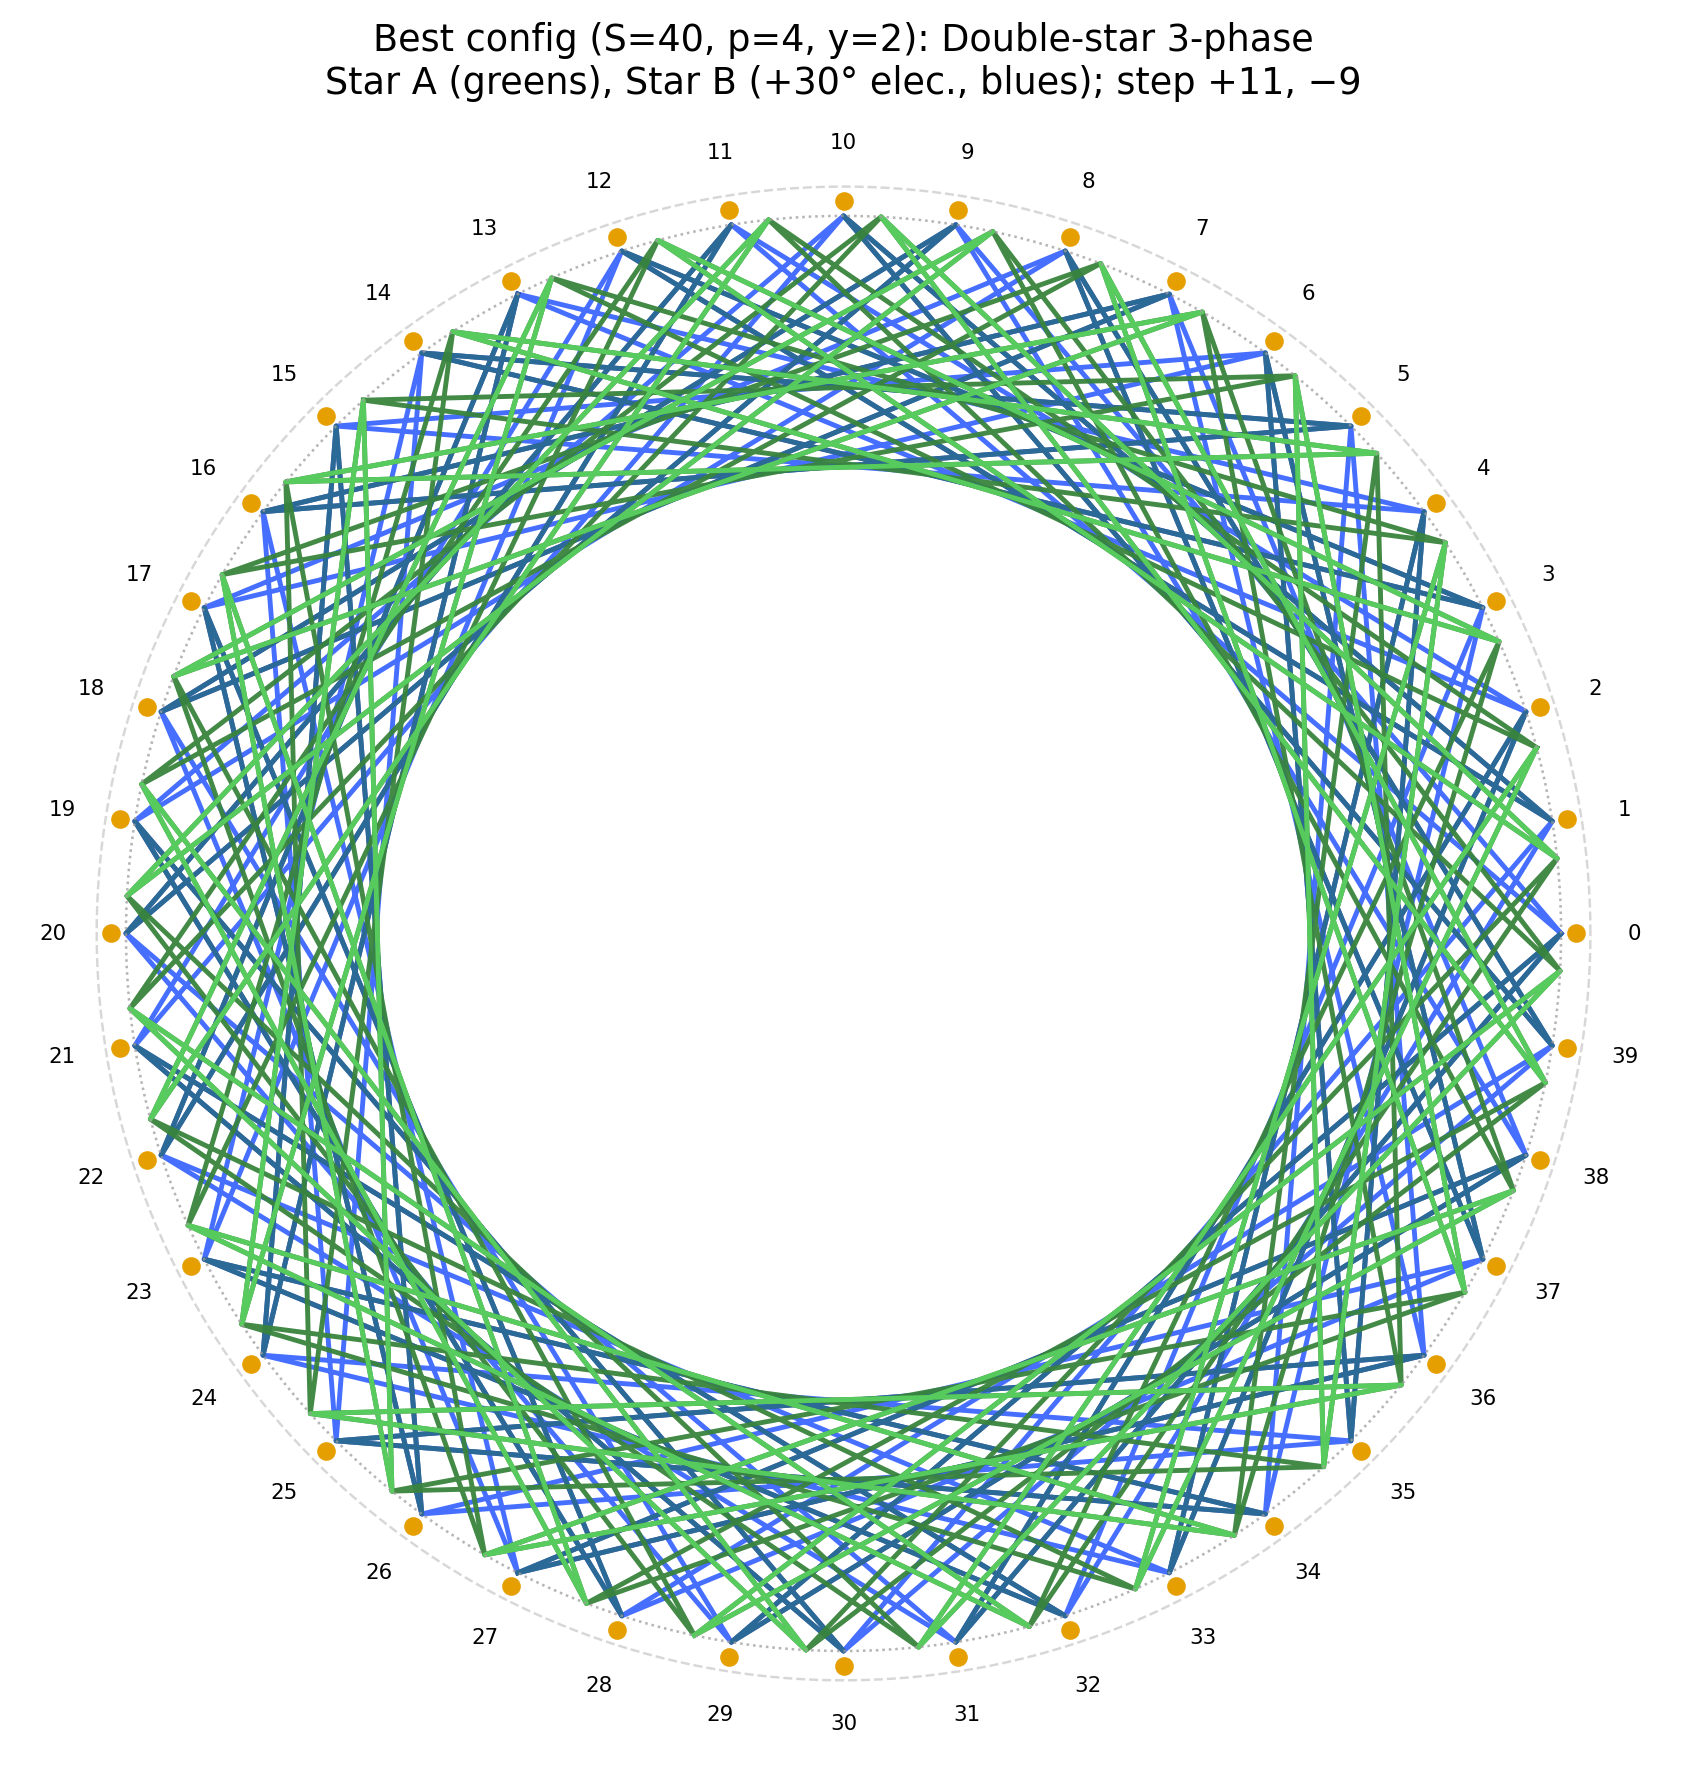
\includegraphics[width=0.7\textwidth]{S40_double_star_best}
\end{center}

\subsection*{Q.2 Stacking (Two Double--Stars)}
Place two identical double--star coils axially stacked (gap $h$).
Let their on--axis contributions be $B_T(z)$ and $B_B(z)$.
Superposition allows the following canonical modes:
\begin{align*}
	\text{Mode A (additive):}&\quad B_{\textrm tot}\simeq B_T+B_B
	\quad\Rightarrow\quad \text{max fundamental}.\\[3pt]
	\text{Mode B (gradient):}&\quad \Delta p = \eta\,\tfrac{B_B^2-B_T^2}{2\mu_0}
	\quad\Rightarrow\quad \text{effective gravity blocking}.\\[3pt]
	\text{Mode C (counter--rot.):}&\quad B_{\textrm rot}\to 0,\;
	\nabla B^2\neq 0
	\quad\Rightarrow\quad \text{standing pressure pattern}.\\[3pt]
	\text{Mode D (beat):}&\quad \varphi\neq 0\;\Rightarrow\;\text{axially traveling envelope}.
\end{align*}

\subsection*{Q.3 Canonical Equation (Swirl Pressure)}
Within SST Canon, the swirl pressure on a foliation slice $\Sigma_t$ is
\[
	p_{\textrm sw}(z) \;=\; \eta\,\frac{\langle B^2(z)\rangle}{2\mu_0},
\]
so that a stacked asymmetry yields
\[
	F_z \;=\; \int_A \Delta p(z)\,dA
	=\eta\;\frac{B_B^2-B_T^2}{2\mu_0}\,A.
\]

\subsection*{Q.4 Experimental Pathway}
\begin{enumerate}
	\item Verify harmonic hygiene: $5^{\textrm th}=0$, $6^{\textrm th}=0$, $7^{\textrm th}\ll1$.
	\item Map $B(z)$ with Hall sensors for both stacks.
	\item Tune $B_B/B_T$ to measure $\Delta p$ on a plate of area $A$.
	\item Switch to Mode~C (counter--rotate top stack) to confirm $\nabla B^2$ persists with vanishing torque.
\end{enumerate}

\subsection*{Q.5 Canonical Status}
This configuration is canonical for coil--based RMF realization in SST:
\begin{itemize}
	\item It implements the harmonic hygiene postulates (Addendum~O).
	\item It realizes swirl pressure modulation in direct accordance with the pressure functional (Canon Core v0.3.3).
	\item It defines a benchmark experimental platform for \emph{gravity--blocking} tests.
\end{itemize}

\subsection*{References}
\begin{thebibliography}{9}
	\bibitem{LandauLifshitzEDCM}
	L.~D. Landau and E.~M. Lifshitz,
	\newblock \emph{Electrodynamics of Continuous Media}, 2nd ed.,
	Pergamon, 1984.

	\bibitem{SimonGeim2000}
	M.~D. Simon and A.~K. Geim,
	``Diamagnetic levitation: Flying frogs and floating magnets (invited),''
	\emph{J. Appl. Phys.}, vol.~87, no.~9, pp. 6200--6204, 2000.
	doi:10.1063/1.372654.

	\bibitem{Batchelor1967}
	G.~K. Batchelor,
	\newblock \emph{An Introduction to Fluid Dynamics},
	Cambridge University Press, 1967.

	\bibitem{Kelvin1869}
	W. Thomson (Lord Kelvin),
	``On Vortex Motion,''
	\emph{Trans. R. Soc. Edinburgh}, vol.~25, pp. 217--260, 1869.
	doi:10.1017/S0080456800028175.
\end{thebibliography}

\bibliographystyle{plain}
\begin{thebibliography}{10}

\bibitem{Aharonov1959}
Y.~Aharonov and D.~Bohm.
\newblock Significance of electromagnetic potentials in the quantum theory.
\newblock {\em Physical Review}, 115(3):485--491, 1959.
\newblock doi:10.1103/PhysRev.115.485.

\bibitem{Tinkham2004}
M.~Tinkham.
\newblock {\em Introduction to Superconductivity}.
\newblock Dover, 2nd edition, 2004.

\bibitem{Onsager1949}
L.~Onsager.
\newblock Statistical hydrodynamics.
\newblock {\em Il Nuovo Cimento (Supplemento)}, 6:279--287, 1949.
\newblock doi:10.1007/BF02780991.

\bibitem{Feynman1955}
R.~P. Feynman.
\newblock Application of quantum mechanics to liquid helium.
\newblock In C.~J. Gorter, editor, {\em Progress in Low Temperature Physics, Vol. I}, pages 17--53. North-Holland, 1955.
\newblock doi:10.1016/S0079-6417(08)60077-3.

\end{thebibliography}

\end{document}